\documentclass{beamer}
\usetheme{Malmoe}
\usecolortheme{seahorse}
\usepackage{pgfplots}
\usepackage{tikz}
\usetikzlibrary{datavisualization}
\usetikzlibrary{datavisualization.formats.functions}

\usepackage{textpos}
\usepackage{csquotes}
\usepackage{listings}
\usepackage{xurl}
\urlstyle{sf}
\usepackage{hyperref}
\usepackage{amsmath}
\usepackage{bm}
\usepackage{textcomp}
\usepackage{caption}
\usepackage{color}
\usepackage{subfigure}
\usepackage{wrapfig}
\usepackage[english]{babel}
\usepackage[backend=biber,style=alphabetic]{biblatex}
\usepackage{mathtools}
\usepackage{subdepth}
\usepackage{graphicx}
\usepackage{blindtext}
\usepackage{svg}
\usepackage{xcolor,colortbl}
\usepackage{media9}
\usepackage{setspace}

\let\oldcite=\cite
\renewcommand{\cite}[1]{\textcolor[rgb]{.55,.55,.89}{\oldcite{#1}}}

\setbeamerfont{frametitle}{size=\small}
\addbibresource{../mscthesis.bib}
\addbibresource{pres.bib}
\captionsetup{justification=raggedright,singlelinecheck=false}

\makeatletter
\AtBeginDocument{%
  \let\l@algorithm\l@lstlisting
  \let\c@algorithm\c@lstlisting
  \let\thealgorithm\thelstlisting
  \renewcommand{\lstlistlistingname}{Algorithms and source code}%
}
\makeatother

\lstdefinelanguage{GLSL}
{
  sensitive=true,
  morekeywords=[1]{
    attribute, const, uniform, varying,
    layout, centroid, flat, smooth,
    noperspective, break, continue, do,
    for, while, switch, case, default, if,
    else, in, out, inout, float, int, void,
    bool, true, false, invariant, discard,
    return, mat2, mat3, mat4, mat2x2, mat2x3,
    mat2x4, mat3x2, mat3x3, mat3x4, mat4x2,
    mat4x3, mat4x4, vec2, vec3, vec4, ivec2,
    ivec3, ivec4, bvec2, bvec3, bvec4, uint,
    uvec2, uvec3, uvec4, lowp, mediump, highp,
    precision, sampler1D, sampler2D, sampler3D,
    samplerCube, sampler1DShadow,
    sampler2DShadow, samplerCubeShadow,
    sampler1DArray, sampler2DArray,
    sampler1DArrayShadow, sampler2DArrayShadow,
    isampler1D, isampler2D, isampler3D,
    isamplerCube, isampler1DArray,
    isampler2DArray, usampler1D, usampler2D,
    usampler3D, usamplerCube, usampler1DArray,
    usampler2DArray, sampler2DRect,
    sampler2DRectShadow, isampler2DRect,
    usampler2DRect, samplerBuffer,
    isamplerBuffer, usamplerBuffer, sampler2DMS,
    isampler2DMS, usampler2DMS,
    sampler2DMSArray, isampler2DMSArray,
  usampler2DMSArray, struct},
  morekeywords=[2]{
    radians,degrees,sin,cos,tan,asin,acos,atan,
    atan,sinh,cosh,tanh,asinh,acosh,atanh,pow,
    exp,log,exp2,log2,sqrt,inversesqrt,abs,sign,
    floor,trunc,round,roundEven,ceil,fract,mod,modf,
    min,max,clamp,mix,step,smoothstep,isnan,isinf,
    floatBitsToInt,floatBitsToUint,intBitsToFloat,
    uintBitsToFloat,length,distance,dot,cross,
    normalize,faceforward,reflect,refract,
    matrixCompMult,outerProduct,transpose,
    determinant,inverse,lessThan,lessThanEqual,
    greaterThan,greaterThanEqual,equal,notEqual,
    any,all,not,textureSize,texture,textureProj,
    textureLod,textureOffset,texelFetch,
    texelFetchOffset,textureProjOffset,
    textureLodOffset,textureProjLod,
    textureProjLodOffset,textureGrad,
    textureGradOffset,textureProjGrad,
    textureProjGradOffset,texture1D,texture1DProj,
    texture1DProjLod,texture2D,texture2DProj,
    texture2DLod,texture2DProjLod,texture3D,
    texture3DProj,texture3DLod,texture3DProjLod,
    textureCube,textureCubeLod,shadow1D,shadow2D,
    shadow1DProj,shadow2DProj,shadow1DLod,
    shadow2DLod,shadow1DProjLod,shadow2DProjLod,
    dFdx,dFdy,fwidth,noise1,noise2,noise3,noise4,
  EmitVertex,EndPrimitive},
  morekeywords=[3]{
    gl_VertexID,gl_InstanceID,gl_Position,
    gl_PointSize,gl_ClipDistance,gl_PerVertex,
    gl_Layer,gl_ClipVertex,gl_FragCoord,
    gl_FrontFacing,gl_ClipDistance,gl_FragColor,
    gl_FragData,gl_MaxDrawBuffers,gl_FragDepth,
    gl_PointCoord,gl_PrimitiveID,
    gl_MaxVertexAttribs,gl_MaxVertexUniformComponents,
    gl_MaxVaryingFloats,gl_MaxVaryingComponents,
    gl_MaxVertexOutputComponents,
    gl_MaxGeometryInputComponents,
    gl_MaxGeometryOutputComponents,
    gl_MaxFragmentInputComponents,
    gl_MaxVertexTextureImageUnits,
    gl_MaxCombinedTextureImageUnits,
    gl_MaxTextureImageUnits,
    gl_MaxFragmentUniformComponents,
    gl_MaxDrawBuffers,gl_MaxClipDistances,
    gl_MaxGeometryTextureImageUnits,
    gl_MaxGeometryOutputVertices,
    gl_MaxGeometryOutputVertices,
    gl_MaxGeometryTotalOutputComponents,
    gl_MaxGeometryUniformComponents,
  gl_MaxGeometryVaryingComponents,gl_DepthRange},
  morecomment=[l]{//},
  morecomment=[s]{/*}{*/},
  morecomment=[l][keywordstyle4]{\#},
}
\lstdefinestyle{GL}{
  tabsize=2,
  rulecolor=,
  basicstyle=\scriptsize,
  upquote=true,
  aboveskip={0.5\baselineskip},
  belowskip={1.5\baselineskip},
  columns=fixed,
  showstringspaces=false,
  extendedchars=true,
  breaklines=true,
  prebreak = \raisebox{0ex}[0ex][0ex]{\ensuremath{\hookleftarrow}},
  frame=single,
  showtabs=false,
  showspaces=false,
  showstringspaces=false,
  identifierstyle=\ttfamily,
  keywordstyle=\color[rgb]{1.0,0,0},
  keywordstyle=[1]\color[rgb]{0,0,0.75},
  keywordstyle=[2]\color[rgb]{0.5,0.0,0.0},
  keywordstyle=[3]\color[rgb]{0.127,0.427,0.514},
  keywordstyle=[4]\color[rgb]{0.4,0.4,0.4}}

\setcounter{biburllcpenalty}{7000}
\setcounter{biburlucpenalty}{8000}

%Information to be included in the title page:

\title{GPU Acceleration of the Material Point Method}

\author % (optional, for multiple authors)
{Fabian Meyer}

\institute % (optional)
{University of Koblenz}

\date{Kolloquium Computergrafik, 14 February 2019}

\begin{document}
\begin{frame}
\titlepage
\end{frame}

\section{Motivation on a GPU MPM Approach}
\subsection{GPGPU for performance enthusiasts}
\begin{frame}
\frametitle{GPGPU for performance enthusiasts}
  Why would('nt) you?
  \vfill
  \begin{columns}[T]
    \begin{column}{0.45\textwidth}
      \textbf{Drawbacks:}
    \begin{itemize}
      \item Interactivity much easier on CPU, but slow PCI-Bus communication
      \item Code is mostly written against GPU architecture
      \item A lot of strain on the programmer
    \end{itemize}
    \end{column}
    \begin{column}{0.45\textwidth}
      \textbf{Benefits:}
    \begin{itemize}
      \item Data is already on the GPU for rendering
      \item \textbf{Higher parallelization acceleration}
    \end{itemize}
    \end{column}
  \end{columns}
\end{frame}

\subsection{A Brief MPM Overview: Do You Want to Build a Snowman?}

\begin{frame}

\frametitle{A Brief MPM Overview: Do You Want to Build a Snowman?}
A short historical summary of MPM:
\vfill
\begin{minipage}{0.43\paperwidth}
  \begin{itemize}
    \item Belongs to family of particle-in-cell(PIC) techniques \cite{evans1957particle}.
    \item Initial application to solids \cite{sulsky1995application} $\rightarrow$ MPM
    \item From research to production in \textit{Disney's} animation film \textit{Frozen} \cite{MPM:SNOW}.
    \item Avalanche research \cite{MPM:AVALANCHE}
  \end{itemize}
\end{minipage}
\begin{minipage}{0.35\paperwidth}
\includemedia[
  width=144,
  height=81,
  activate=pageopen,
  addresource=media/snowh264.mp4,
  flashvars={source=media/snowh264.mp4&autoPlay=true&loop=true&repeat=always}
  ]{\includegraphics{media/snow.jpg}}{VPlayer.swf}
  \tiny{Video result of my bachelor thesis on the simulation of snow \cite{Meyer2015}.}
\end{minipage}
\end{frame}


\begin{frame}
\begin{minipage}{0.45\paperwidth}
PIC ideas:
\begin{itemize}
    \item Particles store all information
    \item Eulerian grid as a non-deformable scratchpad
    \item[$\Rightarrow$] \textbf{meshfree}
\end{itemize}
\vfill
Typical PIC/MPM roundtrip:
\begin{enumerate}
  \item Transfer particle quantities to the grid (\textit{P2G})
  \item Solve discretized governing equations on grid
  \item Transfer back (\textit{G2P})
\end{enumerate}
\end{minipage}
\begin{minipage}{0.30\paperwidth}
\begin{minipage}{1.0\textwidth}
  \small
  \includesvg[width=1.0\textwidth]{media/pic.svg}
  P2G-transfer $\sum_p$
\\
\end{minipage}
\begin{minipage}{1.0\textwidth}
  \small
  \includesvg[width=1.0\textwidth]{media/g2p.svg}
  G2P-transfer $\sum_i$
\end{minipage}
\end{minipage}
\end{frame}
\section{A Gentle Introduction to the MPM}


\subsection{Governing Equations: Conservation of Mass \& Momentum}

\begin{frame}
  \frametitle{Governing Equations: Conservation of Mass \& Momentum}
  \textbf{Conservation of mass}, continuum assumption holds.\\
  Lagrangian (moving with a particle ${}_0\boldsymbol{x}$):
  \begin{equation}
    {^t_0J}\rho(_0\boldsymbol{x},t) = {}\rho(_0\boldsymbol{x},0).
  \end{equation}
Eulerian (outside observer ${}_t\boldsymbol{x}$):
\begin{equation}
  \frac{\partial}{\partial t}\rho(_t\boldsymbol{x},t) = -  \vec{\nabla} \cdot (\rho(_t\boldsymbol{x},t) \boldsymbol{v}(_t\boldsymbol{x},t)).
\end{equation}
Lagrangian and Eulerian view measure differently but give same results. Equations are given in the strong form! \cite{MPM:COURSE}\cite{MIT:CONTINUUM_MECHANICS}
\end{frame}

\begin{frame}
  \textbf{Conservation of momentum}:\\
  Lagrangian (moving with a particle ${}_0\boldsymbol{x}$):
  \begin{equation}
  \rho(_0\boldsymbol{x},0)\boldsymbol{a}(_0\boldsymbol{x},t)
= \vec{\nabla} \cdot \boldsymbol{P}(_0\boldsymbol{x},t) + {\boldsymbol{f}} ^ {\text{body}}(_0\boldsymbol{x},t) {^t_0J}.
  \end{equation}
Eulerian (outside observer ${}_t\boldsymbol{x}$):
\begin{equation}
  \rho(_t\boldsymbol{x},t) \boldsymbol{a}(_t\boldsymbol{x},t) = \vec{\nabla} \cdot \boldsymbol{\sigma}(_t\boldsymbol{x},t) + \boldsymbol{f} ^ {\text{body}}(_t\boldsymbol{x},t)
\end{equation}
Solving this equation will tell us how the velocity fields $\boldsymbol{v}(_t\boldsymbol{x}),\boldsymbol{v}(_0\boldsymbol{x})$ change on the whole domain due to acceleration $\boldsymbol{a}$. This is important to advect particles accounting for all forces. \cite{MPM:COURSE}\cite{MIT:CONTINUUM_MECHANICS}
\end{frame}

\subsection{Discretization of Space and Time}

\begin{frame}
\frametitle{Discretization of Space and Time}
\textbf{Space Discretization} is done in a Galerkin/FEM fashion with grid based interpolants $w_i$. Here dyadic products of cubic b-splines suffice. $w_i$ should satisfy at least \cite{gao2017adaptive}:
\begin{itemize}
  \item Partition of unity: $\sum_i w (\boldsymbol{x}-\boldsymbol{x}^n_i)=1$
  \item Identity relation: $\sum_i \boldsymbol{x}_i w (\boldsymbol{x}-\boldsymbol{x}^n_i)=\boldsymbol{x}$ $(\boldsymbol{x}=\boldsymbol{x}_p)$
  \item Non-negativity: $w \geq 0$.
  \item Limited support.
  \item $C^1$-continuity.
\end{itemize}
Shortening $w^n_{ip} = w(\boldsymbol{x}_p^n - \boldsymbol{x}_i^n).
\begin{tikzpicture}[remember picture,overlay,
  declare function={
    func(\x)= and(abs(\x) >= 0 , abs(\x)<1) * (pow(abs(\x),3)/2 - pow(abs(\x),2) +2/3)  +
	      and(abs(\x) >= 1 , abs(\x)<2) * (1/6* pow((2-abs(\x)),3))
   ;
  }
]
\begin{axis}[
  width=7.5cm,height=3.5cm,
  axis x line=middle, axis y line=middle,
  ymin=-0.1, ymax=1, ytick={0,1}, ylabel=$w$,
  xmin=-2.5, xmax=2.5, xtick={-2,...,2}, xlabel=$x$,
  domain=-2.5:2.5,samples=101, % added
]

\addplot [blue,thick] {func(x)};
\end{axis}
\end{tikzpicture}
\end{frame}

\begin{frame}
Transfer quantities from particles to grid. Numerical integration where the particles function as quadrature points \cite{Steffen}:

$$m_i = \int_\Omega \rho(\boldsymbol{x})w_i(\boldsymbol{x}) d\Omega \approx \sum_p \rho_p w_{ip} V_p \approx \sum_p m_p w_{ip}$$
$$A _ { i } = \int _ { \Omega }  A ( \boldsymbol{x} ) w _ { i } ( \boldsymbol{x} ) d \Omega \approx \sum _ { p } A _ { p }  w_{ip} V _ { p }.$$ \\
\begin{minipage}{0.62\textwidth}
APIC-transfers add a local velocity field $\boldsymbol{C}_p$ around $\boldsymbol{v}_p$:
\\\vspace*{-10}\\
$ ( m \boldsymbol{v} ) _ { i } = \sum _ { p } w _ { i p } m _ { p } \left( \boldsymbol{v} _ { p } + \boldsymbol{C} _ { p } ( \boldsymbol{x} _ { i } - \boldsymbol{x} _ { p } ))$
\end{minipage}
\begin{minipage}{0.33\textwidth}
\begin{minipage}{1.0\textwidth}
  \small
  \includesvg[width=1.0\textwidth]{media/pic.svg}
  P2G-transfer $\sum_p$
\\
\end{minipage}

\end{minipage}
\end{frame}

\begin{frame}
\begin{minipage}{0.64\textwidth}
The MPM can be described in the weak formulation (FEM: virtual quantities). This allows us to 'shift' the derivative:\begin{itemize}
\item $\boldsymbol{A}_p = \sum_i \boldsymbol{A}_i w_{ip} $
\item $\nabla \boldsymbol{A}_p = \sum_i \boldsymbol{A}_i \nabla w_{ip}^T $
\item$\nabla \cdot \boldsymbol{A}_p = \sum_i \boldsymbol{A}^T_i \nabla w_{ip} $
\end{itemize}
\end{minipage}
\begin{minipage}{0.30\textwidth}
\begin{minipage}{1.0\textwidth}
  \small
  \includesvg[width=1.0\textwidth]{media/g2p.svg}
  G2P-transfer $\sum_i$
\end{minipage}
\end{minipage}
\vfill
\textbf{Time discretization} with implicit midpoint scheme:\\
$v_i ^ { n + 1 } - v_i ^ { n } = \frac{\Delta t}{m_i^n}f_i ^ { n + \frac{1}{2} } =\frac{\Delta t}{m_i^n} f \left( t ^ { n } + \frac{\Delta t}{2}, \frac{1}{2} y ^ { n } + \frac{1}{2} y ^ { n + 1 } \right)$
\begin{itemize}
  \item \textbf{implicit} requires linear system solve $\Rightarrow$ more stable, larger time steps
  \item \textbf{midpoint} as it conserves angular momentum
\end{itemize}
\end{frame}
\section{A MPM Guide on GPGPU Pitfalls and Optimizations}
\subsection{Layout of the data: SoA vs. AoS}
\begin{frame}[fragile]
\frametitle{Layout of the data: SoA vs. AoS}

\begin{minipage}{0.31\textwidth}
\begin{minipage}{0.95\textwidth}
Coalescing:
\vspace*{23}
\end{minipage}
\tiny
\begin{minipage}{0.95\textwidth}
  SoA-Layout
\begin{lstlisting}[language={GLSL},style={GL},basicstyle=\tiny]
struct Container{
  vec4 positions[n];
  vec4 velocities[n];
} Particles;
\end{lstlisting}
\vspace*{29}
\end{minipage}
\begin{minipage}{0.95\textwidth}
  AoS-Layout
\begin{lstlisting}[language={GLSL},style={GL},basicstyle=\tiny]
struct Particle {
  vec4 position;
  vec4 velocity;
} Particles[n];
\end{lstlisting}
\end{minipage}
\end{minipage}
\begin{minipage}{0.64\textwidth}
  \tiny
  \includesvg[svgpath =../images/,width=\textwidth]{soa}
  Structures of arrays(SoA)
\\
  \includesvg[svgpath =../images/,width=\textwidth]{aos}
  Arrays of structures(AoS)

\end{minipage}
\end{frame}
\begin{frame}
Nvidia Nsight\cite{NVIDIA:METRICS} now offers metrics to identify bottlenecks:
\vspace{-5}
\begin{table}
  \footnotesize
  \begin{tabular}{ | l | l |}    \hline
    \textbf{Metric}   & \textbf{Description} \\ \hline
    VRAM SOL\%        & memory througput w.r.t. to hardware limit\\\hline
    SM SOL\%          & instruction throughput\\\hline
    L2 SOL\%          & L2-cache throughput\\\hline
    Tex SOL\%         & L1-cache throughput\\\hline
    SM Issue Util.\%  & amount of cycles an instr. was issued\\\hline
  \end{tabular}
\end{table}
\\
\vspace{5}
A simple map(\texttt{y=length(x)}) shader on 1024$\times$1024 Elements SoA vs. AoS differences:
\vspace{-15}
\begin{table}
  \footnotesize
  \begin{tabular}{ | l | l | l | l | l | l | l |}    \hline
    Layout &  $\Delta t_c (\mu s)$	& Speedup &VRAM     & SM     & L2     & SM Issue Util. \\\hline
    AoS(1 instr.)         & 243                   & -       &77.7\%   & 7.3\%  & 30.3\% & 6.8\% \\\hline
    SoA(1 instr.)         & \textbf{120}                   & 2.26x   &75.4\%   & \textbf{14.3}\% & 29.4\% & \textbf{14.0\%} \\\hline
    AoS(2 instr.)         & 275                   & -        &61.3\%           & \textbf{41.8}\% & \textbf{53.8}\% & 48.9\% \\\hline
    SoA(2 instr.)         & 240                   & 1.16x    &75.4\%  & 29.4\%          & 20.0\% & 62.3\% \\
    \hline
\end{tabular}
\end{table}
$\Rightarrow$ SoA increases coalescing for non-random access.
\end{frame}
\subsection{Parallel Reduction \& Scan}
\begin{frame}
\frametitle{Parallel Reduction \& Scan}
Assuming an associative \texttt{binary\_op(x,y)}:= $x \circ y$ , a neutral element $e$ of the \texttt{binary\_op}, and an array of values $\left[a_0,a_1, ... ,a_n\right]$.\\\vspace{10}
\begin{itemize}
  \item \textbf{Parallel reduction} computes the value:
\begin{equation}
  r = a_0 \circ a_1 \circ ... \circ a_n.
\end{equation}
\item (Exclusive) \textbf{scan} computes the array:
\begin{equation}
  \left[e , a_0 , \left(a_0 \circ a_1\right), \left(a_0 \circ a_1 \circ a_2\right), \ ... \ ,\left(a_0\circ a_1 \circ a_2 \circ ...\circ a_{n-1}\right)\right].
\end{equation}
\end{itemize}
\\\vspace{5}
Here, only shared memory approaches without (NVIDIA exclusive) warp shuffle operations.
\end{frame}
\begin{frame}
\textbf{Shared Memory Bank Conflicts}:
\\\vspace{10}
\begin{minipage}{0.94\textwidth}
\begin{minipage}{0.5\textwidth}
  \tiny
  \includesvg[svgpath =../images/,width=1.0\textwidth]{sequential}
  Sequential Addressing
\end{minipage}
\begin{minipage}{0.5\textwidth}
  \tiny
  \includesvg[svgpath =../images/,width=1.0\textwidth]{interleaved}
  Interleaved Addressing
\end{minipage}
\end{minipage}
\\\vspace{10}
\\
Interleaved addressing causes bank conflicts (Short Scoreboard activity) $\Rightarrow$ padding needed.
\vspace{-12}
\begin{table}
    \footnotesize
  \begin{tabular}{ | l | r | r | r | r | r | r | r |}    \hline
    Method         &  $\Delta t_c$ & Speedup &VRAM              & SM              & Sel. Warp-Stall Reas.\\\hline
    Interl. no padd.    & 305                   & -       &23.0\%          & \textbf{60.9}\%  & S. Scoreb.(17.2\%)\\\hline
    Sequential     & 141                   & 2.16x   &\textbf{49.8}\%   & 37.1\%         & \textbf{S. Scoreb.(2.0\%)} \\\hline
  \end{tabular}
    \caption{\footnotesize Parallel reduction on $1024\times1024$ vectors with \texttt{y=length(x)} as input.}
\end{table}
\vspace{-10}
More elements than thread group size require pyramid schemes.
\end{frame}

\begin{frame}

\textbf{Sequential work}: multiple elements per thread.\begin{itemize}
  \item Memory latency hiding (Long Scoreboard up)
  \item Higher reduction factor each dispatch $\Rightarrow$ Less global memory indirections
  \item Unrolling loops can help but adds register pressure.
\end{itemize}
\begin{table}
  \footnotesize
  \begin{tabular}{ | l | r | r | r | r | r | r | r |}    \hline
    Method         &  $\Delta t_c$ & Speedup &VRAM              & SM              & Sel. Warp-Stall Reas.\\\hline
    Sequential     & 141                   & 2.16x   &49.8\%   & 37.1\%         & S. Scoreb.(2.0\%) \\\hline\hline
    Seq. (2x)      & 100                   & 3.05x   &69.5\%            & 26.2\%         & L. Scoreb.(80.1\%)\\\hline
    Seq. (128x)    & 98                    & 3.1x    &\textbf{72.9}\%   & 16.9\%         & \textbf{L. Scoreb.(84.4\%)}\\\hline
    Seq. (256x)    & 101                   & 3.0x    &66.4\%            & 14.6\%         & L. Scoreb.(76.9\%)\\
    \hline
  \end{tabular}
  \caption{\footnotesize Parallel reduction on $1024\times1024$ vectors with \texttt{y=length(x)} as input. Methods have 504, 8, 4 thread groups, respectively. A GTX970 has 13 SMs.}
\end{table}
\vspace{-10}
Scan is similar but cannot profit as much from sequential work having to keep multiple elements in register memory.
\end{frame}
\subsection{Binning \& Counting Sort: Where Are You?}
\begin{frame}
\frametitle{Binning \& Counting Sort: Where Are You?}

Grid node does not know its neighboring particles $\Rightarrow$ Binning.
\\\vspace{10}
Binning combines nicely with \textbf{Counting Sort:}\\
\begin{minipage}{0.55\textwidth}
\begin{enumerate}
  \item \textbf{Binning}: Per node counting.
  \item \textbf{Scan}: Computes new memory offset for particles.
  \item \textbf{Reordering}: Give back indexing list or do deep copy.
\end{enumerate}
\end{minipage}
\begin{minipage}{0.40\textwidth}
  \footnotesize
 \includesvg[svgpath =../images/,width=\textwidth]{binning}
 \caption{\footnotesize Binning: Particle adds one
to counter after storing it as offset.}
 \end{minipage}
\end{frame}

\begin{frame}
Sorting can dramatically increase workload performance of subsequent steps for neighboring queries:
\begin{enumerate}
  \item Deep sorted accesses are now \textbf{coalesced}. \label{it:sort_1}
  \item \textbf{Data reuse} due to L2-Cache and/or shared memory. \label{it:sort_2}
\end{enumerate}
\textbf{Double buffer particles} to use last sorted state as input for new sorting to profit from item 1 and 2!
\begin{table}
  \footnotesize
  \begin{tabular}{ | l | r | r | r | r| r |r|}    \hline
    Ordering            &  $\Delta t_c (\mu s)$ & Speedup &VRAM              & SM      & L2     & L2-Hit \\\hline
    Random              &  1,516                & -       &25.0\%            & 3.4\%   & 9.1\%  & 10.8\% \\\hline
    Deep sorted           &    218                & 6.95x   &\textbf{75.3\%}   & 24.4\%  & \textbf{35.0\%} & \textbf{37.8\%} \\
    \hline
 \end{tabular}
\caption{\footnotesize Order dependency of binning of $1024\times1024$ randomly positioned particles in a $128\times128\times128$ grid.}\label{table:bin}
\end{table}
\end{frame}
\subsection{The MPM Specific Transfers}
\begin{frame}
\frametitle{The MPM Specific Transfers}
All MPM operations belong to one of those parallelization schemes:
\begin{itemize}
 \item 1 thread : 1 particle: $\square_p = \square_p \circ \square_p \circ ... \circ \square_p$.
 \item 1 thread : 1 node: $\square_i = \square_i \circ \square_i \circ ... \circ \square_i$.
 \item G2P-transfer: $\square_p = \sum_i \square_i \circ \square_{ip}.$
 \item P2G-transfer: $\square_i = \sum_p \square_p \circ \square_{ip}.$
\end{itemize}
\vfill
MPM-Transfers are executed \textbf{multiple times per physical frame} with varying numbers of variables and mathematical operations.\\\vspace{5}
$\Rightarrow$ Preprocessing steps only need to be done \textbf{once per physical frame}. Sorting already introduced as one of these.
\end{frame}
\begin{frame}
\begin{minipage}{\textwidth}
  G2P-Transfer: $\square_p = \sum_i \square_i \circ \square_{ip}.$\\
  \includesvg[svgpath =../images/,width=\textwidth]{block_transfer_inv_par}
  Pull-Operations read!
\end{minipage}
\end{frame}
\begin{frame}
Similar to filter or stencil operations on the GPU:
\begin{itemize}
  \item 1 node : 1 thread, split grid into blocks corr. to thread groups.
  \item Interpolation function however dependent on particle position.
  \item Needs to be rerun for every particle in the cell.
\end{itemize}
\vfill
Typical setup of transfers:
\begin{enumerate}
  \item Initialize shared memory (pull: with nodes from global memory).
  \item Perform transfers.
  \item Write back to global memory (push: global atomics since writes on halo).
\end{enumerate}
\end{frame}
\begin{frame}
\begin{minipage}{\textwidth}
  P2G-transfer: $\square_i = \sum_p \square_p \circ \square_{ip}.$\\
  \includesvg[svgpath =../images/,width=\textwidth]{block_transfer_par}
  Pull-Operations read, Push-operations write!\\
  $\Rightarrow$ Race conditions.
\end{minipage}
\end{frame}
\begin{frame}
  Typically simulation domain(grid) much bigger than simulation model. Filtering inactive blocks as a preprocess improves performance.
\begin{itemize}
  \item Block is active if any cell counter is active.
  \item Cell counter is active if it has at least one particle.
\end{itemize}
\vfill
\begin{minipage}{0.9\textwidth}
  \footnotesize
  \includesvg[svgpath =../images/,width=\textwidth]{indirect_dispatch}
\end{minipage}
\end{frame}
\begin{frame}
\begin{itemize}
  \item Block and halo are always target of shared memory operations $\Rightarrow$ P2G-pull low occupancy.
  \item \textbf{Batching} multiple particles can increase performance due to hiding synchronization, unroll!
  \item Transfers respect shared memory bank conflicts fully.
  \item \textbf{Warp divergence} for varying cell counts.
\end{itemize}

{\footnotesize
\begin{table}
  \begin{tabular}{ | l | r | r | r | r | r |}    \hline
    Method                 &  $\Delta t_c(\mu s)$ &Speedup         &VRAM  & L2   &SM     \\\hline
    global                 &   44,442             &-               &4.6 \%&34.4\%&7.7\%  \\\hline
    global sorted          &   20,484		  &2.21x           &7.0 \%&\textbf{44.0}\%&16.1\% \\\hline
    P2G-sync              &    \textbf{2,595}    &17.47x          &5.9\%&7.6\%  &\textbf{67.0}\%\\\hline
 \end{tabular}
\end{table}
P2G-transfers of one uniformly million particles with 4 particles per cell with random velocities between $v_x,v_y,v_z \in [-1.0;1.0]$ in a $128\times 128\times128$ grid. Block size is (8,4,4).
}

\end{frame}
\section{Delving Deeper: Further Opportunities}
\subsection{A comparison to \cite{Gao:2018}}
\begin{frame}
  \frametitle{A comparison to \cite{Gao:2018}}

Simultaneously being worked on. Largely same decision making:\\
\begin{table}
\begin{tabular}{|c|c|c|}
    \hline
	   & \textbf{Me}              & \textbf{\cite{Gao:2018}} \\\hline
  \textbf{Sort}   & Count/Histogram & Count/Histogram \\
	   & for each var.   & sel. variables  \\\hline
  \textbf{Filtering domain}& Filter-op.& Sparse Grid structure \\\hline
  \textbf{Transfers}        & Shared mem. only & Warp-shuffle op.\\\hline
  \end{tabular}
\end{table}
\textbf{Warp shuffle} allows for fast parallel segmented reduction of cells of varying counts.\\
$\Rightarrow$ Solves warp divergence and shared memory issues mostly, thread groups now correspond to particles. Faster for varying counts but \textbf{NVIDIA only}.
\end{frame}
\begin{frame}
  \centering{\textbf{Thank you for your attention!}}
  \vfill
\begin{itemize}
  \item \textbf{Bachelor thesis}: \url{https://github.com/MeyerFabian/snow}
  \item \textbf{Master thesis}: \url{https://github.com/MeyerFabian/msc}
  \item \textbf{Presentation}: \url{https://github.com/MeyerFabian/msc/pres}
      \item \textbf{Code} (right now): \url{https://github.com/mpm-msc/snow}
\end{itemize}
\vfill
\centering
\textbf{Questions?}
\end{frame}

\selectlanguage{english}
\printbibliography

\begin{frame}
\frametitle{The Pretty Strong but Mathematically Weak Formulation}

\textbf{Weak Formulation} (or Principle of Virtual Work):\\
Dot product equations with arbitrarily 'test functions' $\boldsymbol{q}$ and apply divergence theorem:
\begin{align}
\int _ { \Omega ^ { 0 } } _0\boldsymbol{q} \cdot  \Bigl[(_0\rho_0)(_0\boldsymbol{a}) - & {}_0\boldsymbol{f}^{\text{body}}{}_0^tJ\Bigr] d _0\boldsymbol{x}= \nonumber \\
										     &  \int _ { \partial \Omega ^ { t^n } } _t\boldsymbol{q} \cdot \boldsymbol{\sigma} d_t\boldsymbol{A} - \int _ { \Omega ^ { t^n} } \nabla {}_t\boldsymbol{q} : \boldsymbol{\sigma}  d_t\boldsymbol{x}.
\end{align}
A strong solution is also a solution to the weak formulation. Leave out body forces(like gravity) and boundary condition (e.g. collisions) for now:
\begin{equation}
  \int _ { \Omega ^ { 0 } } _0\boldsymbol{q} \cdot (_0\rho_0)(_0\boldsymbol{a}) d _0\boldsymbol{x}= \int _ { \Omega ^ { t^n} } \nabla {}_t\boldsymbol{q} : \boldsymbol{\sigma}  d_t\boldsymbol{x}.
\end{equation}
\end{frame}
\begin{frame}[fragile]
\textbf{Weak Derivative}:
\vfill
\begin{minipage}{0.49\textwidth}
  $y=|t|$ has weak derivative:
  \\\\
$ v = \left\{ \begin{array} { l l }
{ - 1 , } & { \text { if } t < 0 } \\
{ c , } & { \text { if } t = 0 } \\
{ 1 , } & { \text { if } t > 0 }
\end{array} \right.$
\\

\end{minipage}
\begin{minipage}{0.4\textwidth}
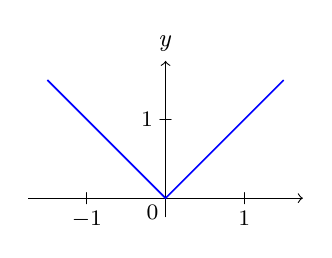
\begin{tikzpicture}
  \small
\datavisualization [school book axes,
		    y axis = {attribute = y, label},
		    visualize as line/.list={fx},
		    fx={style={color=blue}}
]

data [set=fx,format=function] {
      var x : interval [-1.5:1.5] samples 5;
      func y = abs(\value x);
      };
\end{tikzpicture}
\end{minipage}

\vfill
\begin{minipage}{0.49\textwidth}
  Heaviside step function has no weak derivate: \\\\
  $s= \left\{ \begin{array} { l l } { 0 , } & { \text { if } t < 0 } \\ { 1 , } & { \text { if } t \geq 0 } \end{array} \right.$
\end{minipage}
\begin{minipage}{0.4\textwidth}
\begin{tikzpicture}
  \small
  \begin{axis}[axis lines = middle, width=5.1cm,height=3.5cm,xtick={-1,0,1},ytick={0,1},ymin=-0.3,ymax=1.25,xmin=-1.8,xmax=1.8,ylabel=$s$]
                \addplot[blue,mark=*,mark options={fill=white},samples at={-2.1,0}] {0};
                \addplot[blue,mark=*,samples at={0,2.1}] {1.0};
            \end{axis}
\end{tikzpicture}
\end{minipage}
\vfill
Allows for point loads, material discontinuities and more. \cite{bathe2006finite}
\end{frame}

\begin{frame}[fragile]
\textbf{Space Discretization} is done in a Galerkin/FEM fashion with grid based interpolants $w_i$ with limited support. Here dyadic products
\begin{equation}
  w_i(\boldsymbol{x}) =w(\boldsymbol{x}-\boldsymbol{x}_i) = w(\frac{1}{h}(x-x_i))w(\frac{1}{h}(y-y_i)w(\frac{1}{h}(z-z_i))
\end{equation}
of cubic b-splines suffice:
\begin{equation}
w ( x ) = \left\{ \begin{array} { l l } { \frac { 1 } { 2 } | x | ^ { 3 } - | x | ^ { 2 } + \frac { 2 } { 3 } } & { 0 \leqslant | x | < 1 } \\ { \frac { 1 } { 6 } ( 2 - | x | ) ^ { 3 } } & { 1 \leqslant | x | < 2 } \\ { 0 } & { 2 \leqslant | x | } \end{array}. \right
\end{equation}
\begin{tikzpicture}[
  declare function={
    func(\x)= and(abs(\x) >= 0 , abs(\x)<1) * (pow(abs(\x),3)/2 - pow(abs(\x),2) +2/3)  +
	      and(abs(\x) >= 1 , abs(\x)<2) * (1/6* pow((2-abs(\x)),3))
   ;
  }
]
\begin{axis}[
  width=10cm,height=4cm,
  axis x line=middle, axis y line=middle,
  ymin=-0.1, ymax=1, ytick={0,1}, ylabel=$w$,
  xmin=-2.5, xmax=2.5, xtick={-2,...,2}, xlabel=$x$,
  domain=-2.5:2.5,samples=101, % added
]

\addplot [blue,thick] {func(x)};
\end{axis}
\end{tikzpicture}
\end{frame}
\section*{Rest}
\end{document}
